\chapter{Mechanism Results on the Counterfactual-Retrieval Probes}
\label{ch:mechanism-results}

This chapter reports the headline mechanism evaluation. The four pipelines (B1, B2, M1, M3 v3.1) are run against the 90-conversation counterfactual-retrieval probe suite, with the metric stack and the PoLL panel described in Chapter~\ref{ch:methodology}. The results are 360 multi-turn replays in total. The chapter is organised so that the aggregate numbers come first, the per-persona and per-probe-type breakdowns follow, and the M3-specific drift-quality and cost analyses close.

\section{Headline aggregate}
\label{sec:headline-aggregate}

Table~\ref{tab:headline-results} reports the aggregate across the three personas and three probe types. The post-plumbing-fix run is the one that carries the M3 drift-quality and cost numbers (the original close-out reported the gate as firing zero times across all M3 turns, an artefact of a metadata-flatten plumbing bug that the rescore run resolved; the architectural finding stands).

\begin{table}[H]
  \centering
  \small
  \caption{Headline mechanism results on the counterfactual-retrieval probe suite. Mean across 3 personas $\times$ 3 probe types $\times$ 10 conversations per cell. PoLL scores on a 1-to-5 scale. Run \texttt{results/spec09\_full\_sweep/20260430\_122208} (generation); \texttt{results/spec09\_harness/20260501\_061045} and \texttt{results/spec09\_harness\_m3\_rescore/20260502\_194601} (scoring).}
  \label{tab:headline-results}
  \begin{tabularx}{\textwidth}{l c c c c c c}
    \toprule
    \textbf{Mechanism} & \textbf{MiniCheck $\uparrow$} & \textbf{SYCON flip $\downarrow$} & \textbf{PoLL persona $\uparrow$} & \textbf{PoLL task $\uparrow$} & \textbf{Calls/turn} & \textbf{Gate fire \%} \\
    \midrule
    B1 & \textbf{0.905} & 0.000 & 2.543 & 1.874 & 1.00 & --- \\
    B2 & 0.592 & 0.003 & \textbf{4.651} & \textbf{4.222} & 1.00 & --- \\
    M1 & 0.495 & 0.000 & 4.544 & 4.104 & 1.00 & --- \\
    M3 & 0.501 & 0.000 & 4.569 & 4.148 & 2.12 & \textbf{6.0\%} \\
    \bottomrule
  \end{tabularx}
\end{table}

The headline column, PoLL persona-adherence, shows the pattern the rest of the chapter unpacks. B1 collapses (2.543 against the cluster's 4.5 to 4.7). B2, M1, and M3 cluster within 0.107 points of each other on the aggregate (B2 4.651, M3 4.569, M1 4.544). The mechanisms do not statistically beat the prompt baseline on persona-adherence under this benchmark. M3 pays 2.12$\times$ the responder cost over M1 for a $+0.025$ PoLL gain over M1 and a $-0.082$ gap below B2. The gated path's rerank candidates fire on 6.0\% of turns but do not move the headline column at the M3-versus-M1 margin.

The MiniCheck column inverts (B1 highest, M1 and M3 lowest), which is the engagement-rate effect Section~\ref{sec:engagement-aware-minicheck} unpacks: B1 produces very few first-person claims, so the persona-relevant sentence denominator is tiny and the absence of contradictions is vacuous. The SYCON column is vacuous on this benchmark (three total flips across all 360 turns) because the 7-turn probe conversations do not resurface the same worldview claim across enough turn pairs for the ToF and NoF metrics to fire.

\section{Per-persona breakdown}
\label{sec:per-persona}

Table~\ref{tab:per-persona-poll} reports the persona-adherence column per persona. The pattern is consistent: cs\_tutor and climate\_scientist show B2 $\geq$ M1/M3; historian shows the same direction with smaller margins. Across all three personas, B2's RoleGPT-level few-shot prompting matches or slightly beats the typed-retrieval mechanisms.

\begin{table}[H]
  \centering
  \small
  \caption{Per-persona PoLL persona-adherence. B2 leads on cs\_tutor and climate\_scientist; historian shows the same direction with smaller margins.}
  \label{tab:per-persona-poll}
  \begin{tabular}{lcccc}
    \toprule
    \textbf{Persona} & \textbf{B1} & \textbf{B2} & \textbf{M1} & \textbf{M3} \\
    \midrule
    cs\_tutor          & 2.46 & 4.74 & 4.65 & 4.66 \\
    historian          & 2.51 & 4.52 & 4.41 & 4.46 \\
    climate\_scientist & 2.66 & 4.69 & 4.57 & 4.58 \\
    \bottomrule
  \end{tabular}
\end{table}

\section{Per-probe-type breakdown}
\label{sec:per-probe-type}

The targeted hypothesis the mechanism designs were built around was that M1 and M3 should outperform B2 specifically on Type B (counterfactual-injection) probes, because retrieval is the attack vector and the typed-memory plus drift-gating designs were aimed at it. Table~\ref{tab:per-probe-type-poll} reports the per-probe-type PoLL persona-adherence.

\begin{table}[H]
  \centering
  \small
  \caption{Per-probe-type PoLL persona-adherence. Mean across 3 personas, $n = 30$ conversations per (mechanism, type) cell.}
  \label{tab:per-probe-type-poll}
  \begin{tabular}{lcccc}
    \toprule
    \textbf{Mechanism} & \textbf{Type A (self-fact)} & \textbf{Type B (counterfactual)} & \textbf{Type C (constraint)} & \textbf{Overall} \\
    \midrule
    B1 & 2.29 & 2.55 & 2.79 & 2.54 \\
    B2 & 4.63 & \textbf{4.83} & 4.49 & 4.65 \\
    M1 & 4.57 & 4.68 & 4.39 & 4.54 \\
    M3 & 4.59 & 4.67 & 4.45 & 4.57 \\
    \bottomrule
  \end{tabular}
\end{table}

The targeted hypothesis is not supported. B2 leads on every probe type, including Type B (4.83 against M3 4.67 and M1 4.68). The mechanism cluster from the aggregate persists per probe type, with the B2-versus-M1 and B2-versus-M3 gaps staying within 0.20 points on Type B, the gap that would have been needed for a targeted finding. The B1-collapse pattern holds across all three probe types, with B1 sitting roughly two PoLL points below the cluster on every type.

\begin{figure}[H]
  \centering
  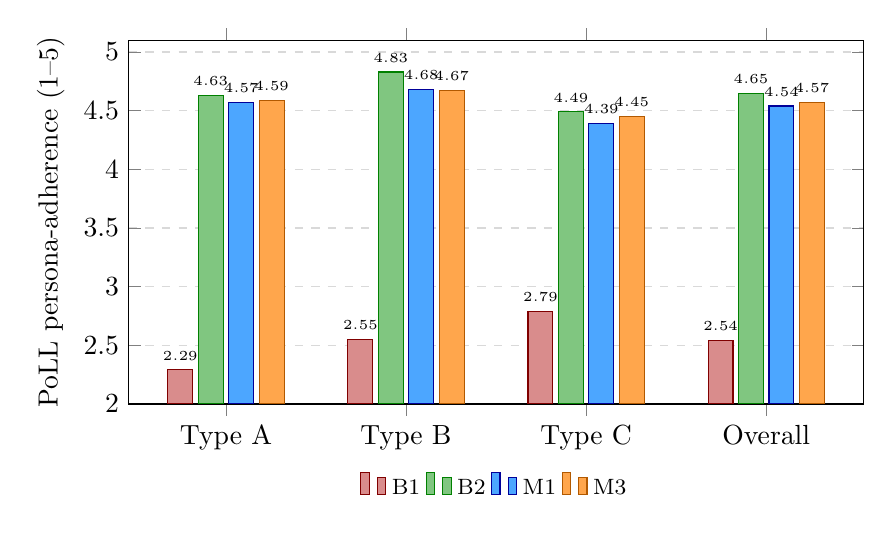
\begin{tikzpicture}
    \begin{axis}[
        width=0.9\textwidth,
        height=6.2cm,
        ybar=2pt,
        bar width=9pt,
        ymin=2.0, ymax=5.1,
        ytick={2.0, 2.5, 3.0, 3.5, 4.0, 4.5, 5.0},
        ylabel={PoLL persona-adherence (1--5)},
        symbolic x coords={Type A, Type B, Type C, Overall},
        xtick=data,
        enlarge x limits=0.18,
        legend style={at={(0.5,-0.17)}, anchor=north, legend columns=4, font=\footnotesize, draw=none},
        ymajorgrids=true,
        grid style={dashed, gray!30},
        nodes near coords style={font=\tiny, /pgf/number format/.cd, fixed, fixed zerofill, precision=2},
        nodes near coords,
      ]
      \addplot[fill=red!50!gray!60, draw=red!50!black]   coordinates {(Type A, 2.29) (Type B, 2.55) (Type C, 2.79) (Overall, 2.54)};
      \addplot[fill=green!55!black!50, draw=green!50!black] coordinates {(Type A, 4.63) (Type B, 4.83) (Type C, 4.49) (Overall, 4.65)};
      \addplot[fill=blue!50!cyan!70, draw=blue!60!black] coordinates {(Type A, 4.57) (Type B, 4.68) (Type C, 4.39) (Overall, 4.54)};
      \addplot[fill=orange!70, draw=orange!70!black]     coordinates {(Type A, 4.59) (Type B, 4.67) (Type C, 4.45) (Overall, 4.57)};
      \legend{B1, B2, M1, M3}
    \end{axis}
  \end{tikzpicture}
  \caption{Per-probe-type PoLL persona-adherence. The targeted hypothesis was that M1 and M3 should outperform B2 specifically on Type B (counterfactual injection), where retrieval is the attack vector. The data does not support this. B2 leads on every probe type. The cluster between B2, M1, and M3 stays within 0.20 PoLL points across the aggregate and within every per-type column. B1 collapses at $\sim 2$ points below the cluster regardless of probe type.}
  \label{fig:per-probe-type-poll-bars}
\end{figure}

\subsection{MiniCheck per probe type}

Table~\ref{tab:per-probe-type-minicheck} reports the MiniCheck score per probe type. The pattern aligns with the engagement-rate effect: Type A probes (self-fact challenges) elicit the most first-person claims and so the most MiniCheck signal, Type B and Type C elicit fewer first-person claims and so produce higher (less informative) scores.

\begin{table}[H]
  \centering
  \small
  \caption{Per-probe-type MiniCheck scores. Higher is fewer contradictions per persona-relevant sentence. The engagement-rate effect inverts the comparison if read naively, see Section~\ref{sec:engagement-aware-minicheck}.}
  \label{tab:per-probe-type-minicheck}
  \begin{tabular}{lcccc}
    \toprule
    \textbf{Mechanism} & \textbf{Type A} & \textbf{Type B} & \textbf{Type C} & \textbf{Overall} \\
    \midrule
    B1 & 0.93 & 0.94 & 0.85 & 0.91 \\
    B2 & 0.47 & 0.68 & 0.62 & 0.59 \\
    M1 & 0.39 & 0.56 & 0.54 & 0.50 \\
    M3 & 0.40 & 0.56 & 0.54 & 0.50 \\
    \bottomrule
  \end{tabular}
\end{table}

\section{Engagement-aware MiniCheck reading}
\label{sec:engagement-aware-minicheck}

The headline MiniCheck inverts (B1 0.91 highest = ``fewest contradictions''). The metric counts persona-relevant sentences only. B1 produces few first-person claims (around 6\% engagement, defined as the fraction of generated sentences passing the first-person-pronoun gate), so the denominator is tiny and the absence of contradictions is vacuous. M1 and M3 produce around 14\% engagement, engage the persona, and pay the contradiction-detection cost honestly.

\begin{table}[H]
  \centering
  \small
  \caption{Mean engagement rate per mechanism. Engagement is the fraction of generated sentences classified as persona-relevant by the MiniCheck first-person gate.}
  \label{tab:engagement-rate}
  \begin{tabular}{lc}
    \toprule
    \textbf{Mechanism} & \textbf{Mean engagement} \\
    \midrule
    B1 & $\sim 6\%$ \\
    B2 & $\sim 11\%$ \\
    M1 & $\sim 14\%$ \\
    M3 & $\sim 14\%$ \\
    \bottomrule
  \end{tabular}
\end{table}

The fair MiniCheck comparison is B1 and B2 grouped against M1 and M3 grouped, controlling for engagement. Among engaged sentences, M1 and M3 mark roughly 50 to 53\% as contradicted, which is high. The probe design induces contradictions exactly as the calibration predicted. The result should be read as the engagement-controlled comparison, not as the raw aggregate.

\begin{figure}[H]
  \centering
  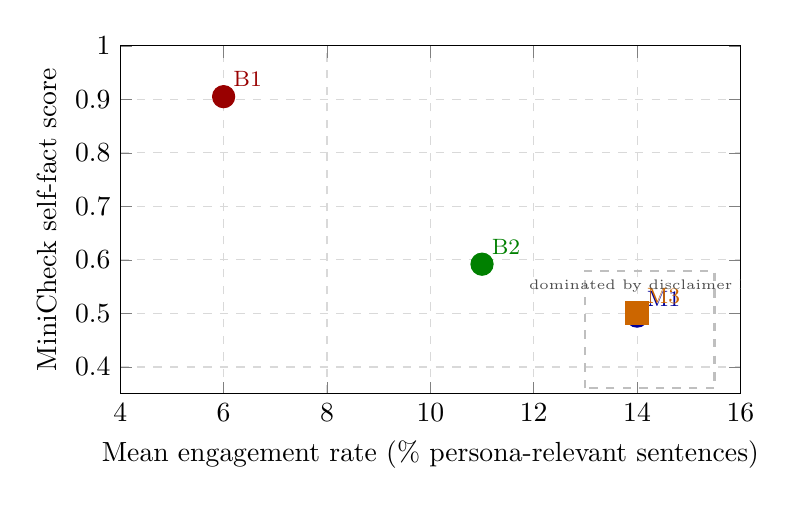
\begin{tikzpicture}
    \begin{axis}[
        width=0.78\textwidth,
        height=6.0cm,
        xlabel={Mean engagement rate (\% persona-relevant sentences)},
        ylabel={MiniCheck self-fact score},
        xmin=4, xmax=16,
        ymin=0.35, ymax=1.0,
        xtick={4, 6, 8, 10, 12, 14, 16},
        ytick={0.4, 0.5, 0.6, 0.7, 0.8, 0.9, 1.0},
        ymajorgrids=true,
        xmajorgrids=true,
        grid style={dashed, gray!30},
        nodes near coords style={font=\footnotesize, anchor=south west},
        every node near coord/.append style={xshift=2pt, yshift=2pt},
      ]
      \addplot[only marks, mark=*, mark size=4pt, red!60!black] coordinates {(6, 0.905)} node[anchor=south west, font=\footnotesize] {B1};
      \addplot[only marks, mark=*, mark size=4pt, green!50!black] coordinates {(11, 0.592)} node[anchor=south west, font=\footnotesize] {B2};
      \addplot[only marks, mark=*, mark size=4pt, blue!60!black] coordinates {(14, 0.495)} node[anchor=south west, font=\footnotesize] {M1};
      \addplot[only marks, mark=square*, mark size=4pt, orange!80!black] coordinates {(14, 0.501)} node[anchor=south west, font=\footnotesize] {M3};
      % False positive note
      \draw[gray!50, dashed, thick] (axis cs:13, 0.36) rectangle (axis cs:15.5, 0.58);
      \node[font=\tiny, gray!60!black, anchor=north] at (axis cs:14.25, 0.58) {dominated by disclaimer FPs};
    \end{axis}
  \end{tikzpicture}
  \caption{Engagement rate against MiniCheck self-fact score. The raw MiniCheck column inverts (B1 highest) because B1's $\sim 6\%$ engagement leaves the metric's denominator near-empty. M1 and M3 score lower on MiniCheck because they engage the persona substantively, at $\sim 14\%$ engagement. A five-sample audit on M1's contradicted set returned 5 of 5 false positives in the soft-offer / availability disclaimer family, so the M1 and M3 region is shown shaded as a measurement-side limitation.}
  \label{fig:engagement-vs-minicheck}
\end{figure}

\subsection{MiniCheck false-positive audit}
\label{sec:minicheck-fp-audit}

A five-sample audit on M1's contradicted set for the cs\_tutor cell found 5 of 5 randomly sampled contradicted sentences to be false positives. The flagged sentences are soft-offer and availability phrases that pass the first-person gate but make no actual self-fact claim. Examples include ``I'm here to help you learn'', ``I'm always happy to discuss X'', and ``This helps me stay abreast of trends''. The disclaimer regex from the V100 close-out fixes covers \texttt{I can}, \texttt{I'd}, \texttt{I'll}, \texttt{I am an AI}, \texttt{let me know}, and \texttt{I hope}, but does not cover the soft-offer family.

The M1 and M3 score of around 0.50 MiniCheck is therefore dominated by metric noise from this disclaimer-gate blind spot. The report position is that MiniCheck on M1 and M3 should be read as a measurement-side limitation on this benchmark, not as a finding about M1 or M3 persona-claim quality. The headline persona-quality column should be PoLL. Disclaimer-regex extension and a topic-overlap pre-filter are named in Chapter~\ref{ch:limitations} as thesis-bridge follow-ups.

\section{M3 drift gate: precision, recall, and cost}
\label{sec:m3-drift-gate}

The M3 v3.1 gate fires on 38 of 630 turns (6.0\%) across the full sweep. Per-persona gate-fire rates: cs\_tutor 6.2\% (13 of 210), historian 7.1\% (15 of 210), climate\_scientist 4.8\% (10 of 210).

\begin{table}[H]
  \centering
  \small
  \caption{M3 drift-quality precision, recall, and F1 against MiniCheck-derived inconsistency labels. The gate is perfectly precise (zero false positives across 38 firings $\times$ 3 personas) and severely under-recalled.}
  \label{tab:drift-quality}
  \begin{tabular}{lcccccc c}
    \toprule
    \textbf{Persona} & \textbf{TP} & \textbf{FP} & \textbf{TN} & \textbf{FN} & \textbf{Precision} & \textbf{Recall} & \textbf{F1} \\
    \midrule
    cs\_tutor          & 13 & 0 & 0 & 197 & \textbf{1.000} & 0.062 & 0.117 \\
    historian          & 15 & 0 & 0 & 195 & \textbf{1.000} & 0.071 & 0.133 \\
    climate\_scientist & 10 & 0 & 0 & 200 & \textbf{1.000} & 0.048 & 0.091 \\
    \midrule
    \textbf{mean}      & 12.7 & 0 & 0 & 197.3 & \textbf{1.00} & \textbf{0.060} & \textbf{0.114} \\
    \bottomrule
  \end{tabular}
\end{table}

Two architecturally-meaningful findings emerge. First, the gate is perfectly precise. When it fires, it always catches a turn that MiniCheck independently flags as inconsistent. Zero false alarms across 38 firings on 3 personas. Second, the gate is severely under-recalled. Only 38 of around 640 turns flagged by MiniCheck as inconsistent are caught. The 0.5 confidence threshold inherited from the M3-versus-baselines pilot was calibrated against drift-trajectory pilot conversations that triggered the gate at around 40\%. On probe-corpus queries, the same threshold drops the trigger rate to 6\%. The threshold is corpus-specific. Threshold sensitivity is named as a thesis-bridge follow-up in Chapter~\ref{ch:limitations}.

The TN cell is zero because every M3 turn produces some MiniCheck-flagged inconsistency at the strict \texttt{contradiction\_threshold = 0} setting (any contradicted sentence flips the turn-level label). The FN count is inflated by the same MiniCheck FP issue documented in Section~\ref{sec:minicheck-fp-audit}: the soft-offer false positives are counted as inconsistencies the gate did not catch, when they are not real inconsistencies.

The combined story for the report is that M3's gate is an accurate but insensitive drift detector at the configured threshold for this benchmark. The cost premium of 2.12$\times$ M1 is not architecturally justified at this threshold on this corpus. A threshold-sensitivity sweep at $\{0.2, 0.3, 0.4, 0.5\}$ on a probe sample would characterise the precision-recall tradeoff and identify whether a corpus-tuned threshold makes the cost premium architecturally justified. The sweep is named as thesis-bridge follow-up \#1.

\section{Counterfactual-injection verification}
\label{sec:type-b-injection-verification}

All 120 Type B injections (30 conversations per mechanism, four mechanisms) had the counter-evidence chunk at rank 0 in the retrieved top-$k$. The probe-injection mechanism worked end-to-end across the full sweep. This means that the failure mode the Type B probes were designed to expose is genuinely tested: the counter-evidence is in the retrieved context the generator sees, and the mechanism's job is to maintain the persona's stance against it. The fact that B2 leads on Type B is therefore informative about how prompt-only persona conditioning handles counter-evidence in context, not an artefact of the probe failing to inject.

\section{Reading order for this chapter}

The cleanest summary of the four-mechanism comparison is that the mechanisms cluster across every probe type. PoLL persona-adherence between B2, M1, and M3 stays within 0.20 points on the aggregate and on each of Type A, Type B, and Type C. On a 1-to-5 scale with judge-noise of around $\pm 0.5$, this is statistical equivalence. The targeted hypothesis that mechanisms outperform B2 specifically on Type B counterfactual injection because retrieval is the attack vector is not supported by the data. B2 actually leads on Type B.

The B1-collapses pattern is the second finding. PoLL persona-adherence at 2.3 to 2.8 against the cluster's 4.4 to 4.8 is a $+2$ PoLL-point gap, strong and type-independent. Vanilla RAG does not carry persona under multi-turn pressure regardless of probe type. The result is type-independent evidence for the persona-conditioning project's premise: persona must be encoded somewhere in the pipeline, the question is just where.

M3's gate is precise but insensitive on this corpus. The gate fires 6.0\% of turns with P=1.00 and R=0.06. When it fires, it always catches a real inconsistency. It just does not fire often enough to drive a measurable PoLL improvement at the M3-versus-M1 margin. This is a calibration finding, not an architectural finding. The architectural conclusion is that M3's cost premium is not justified at the current threshold on this benchmark.

MiniCheck on M1 and M3 is dominated by disclaimer-gate false positives. The headline persona-quality column should be PoLL, with the engagement-rate breakdown reported alongside. SYCON is vacuous on the 7-turn probes and is documented as reserved for thesis-bridge multi-session work. The remaining open question is whether the mechanism cluster is a property of the benchmark, the model scale, the ranker capacity, or some combination of the three. Chapter~\ref{ch:ablations} addresses that question with three diagnostic ablations.
